% !TEX root = ../main.tex
\section{Access loss under four typhoons}
\label{sec:access}

\textbf{Baseline.} \cellsPopM{} people live in the 1~km cells. On the network, \routeShare{} of them have a road or ferry route to one of \nHosp{} hospitals, with a population-weighted mean trip of \meanHours{}~h; the raster reaches \rasterReach{} with a mean of \rasterHours{}~h. Results are also written for \nAdmThree{} municipalities. Figure~\ref{fig:network} shows the ferry routes and hospitals.

\begin{figure}[htbp]
\centering
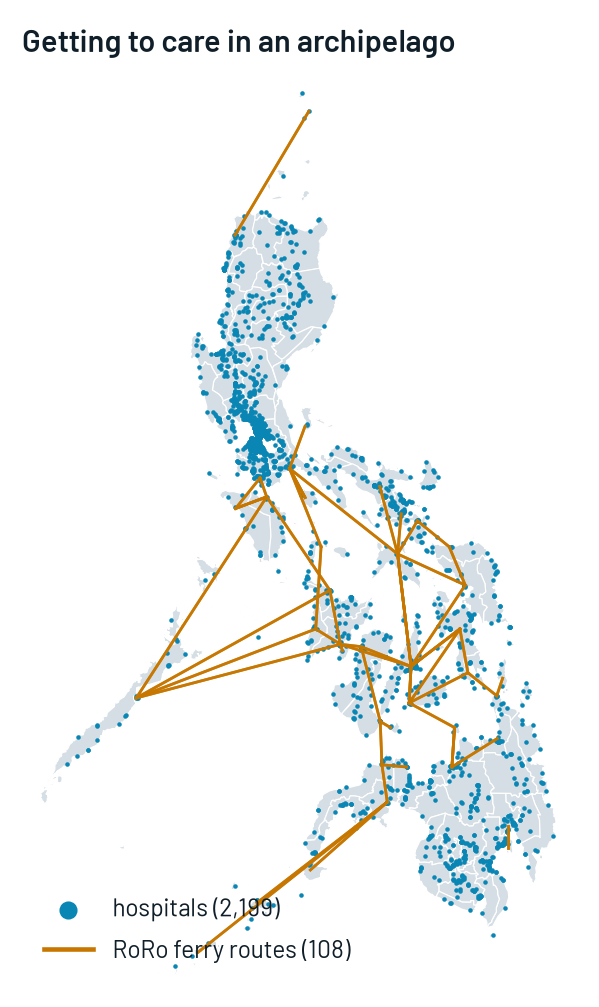
\includegraphics[width=0.45\linewidth]{f13_network}
\caption{Getting to care in an archipelago: the ferry routes (2024--2026 operations, a proxy for 2018--2020) and the fallback hospital list.}
\label{fig:network}
\end{figure}

Table~\ref{tab:methods} gives the people cut off by each method for the observed tracks, and Figure~\ref{fig:access} maps the network's access loss $A$ per unit.

\begin{table}[htbp]
\centering
\caption{People cut off per observed track: network, raster and the range of the per-unit minimum and maximum of the two; rank agreement of $A$ over units ($\rho$) and of $P$ (Kendall's $\tau$); top-ten provinces by $P$ shared; vulnerable people cut off (network).}
\label{tab:methods}
\footnotesize
\begin{tabular}{@{}l r r r r r r r r@{}}
\toprule
typhoon & network & raster & range & $\rho$ of $A$ & $\tau$ of $P$ & top-10 shared & under-5 & 60+ \\
\midrule
\tablerows{methods}
\bottomrule
\end{tabular}
\end{table}

\begin{figure}[htbp]
\centering
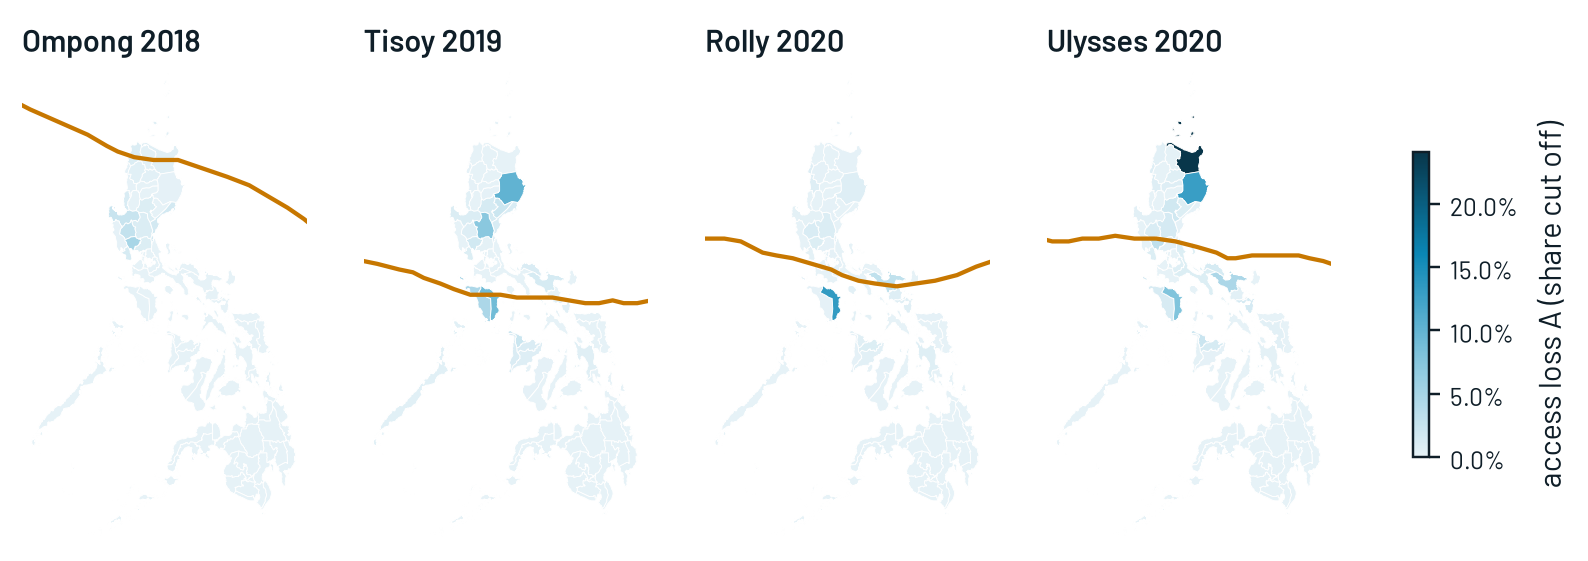
\includegraphics[width=\linewidth]{f08_access}
\caption{Network access loss $A$ per unit for the observed tracks. Roads are cut by Sentinel-1 observed flood; ferries crossing the gale swath are cancelled.}
\label{fig:access}
\end{figure}

\begin{note}
Observed tracks: roads are cut only where Sentinel-1 saw new water. Radar misses floods under dense vegetation, in built-up areas and between passes, so these are \textbf{lower bounds}. The \nProxy{} shifted tracks have no image and use the NOAH 25-year proxy (every high-hazard road in the swath cut): \proxyCutRange{} people cut off on the network, an \textbf{upper bound}. Ferry routes are 2024--2026 operations, a proxy for 2018--2020. $A$ uses radar that exists up to \sOneAfterDays{} days after the forecast origin: it is a retrospective access estimate.
\end{note}

\subsection{Network against friction raster}

The proposal runs a raster method next to the network because OSM completeness is uneven, and reports their disagreement as uncertainty. Both use the same hospitals, population cells, ferry lines and storm rules.

\textbf{On a normal day} the raster reaches \ifRasterReachMore more\else fewer\fi{} people (\rasterReach{} against \networkReach{}) and is \ifRasterFaster faster\else slower\fi{} (population-weighted mean \rasterHours{}~h against \networkHours{}~h; median cell ratio of raster to network \medianRatioBase{})\ifRasterFaster: it can cross land without a mapped road\fi. The two rank places \ifMethodsRankAlike alike\else differently\fi: Spearman \spearmanCells{} over the \cellsBoth{} cells that both reach, and \spearmanUnits{} over the \nUnits{} units' mean trip.

\textbf{Under a storm} (Figure~\ref{fig:methods}), with Sentinel-1 flood the raster cuts off \ifRasterMoreSOne more\else fewer\fi{} people than the network (\cutRasterRange{} against \cutNetRange{}); with the NOAH proxy it cuts off \ifRasterMoreProxy more\else fewer\fi{} (median ratio \proxyRatio{}).\ifRasterMoreSOne\ifRasterMoreProxy\else{} The gap changes sign with the flood source. A likely reason: at 1~km a flooded cell centre closes the whole cell, while radar flood is patchy and the network closes only the flooded road edges; the proxy closes every high-hazard road, which the raster's cell-centre test samples more sparsely.\fi\fi{} The unit rankings of $A$ have $\rho$ \rhoProxyRange{} under the proxy and \rhoObsRange{} with radar\ifProxyAgreesBetter{} (they agree better under the proxy)\fi, and with radar \topTenSharedRange{} of the top-ten provinces by $P$ are shared. The dashboard shows $A$ and $P$ with this range. On the raster method the sensitivity analysis of Section~\ref{sec:validation} gives Kendall's $\tau \geq \tauMinRaster$.

\begin{figure}[htbp]
\centering
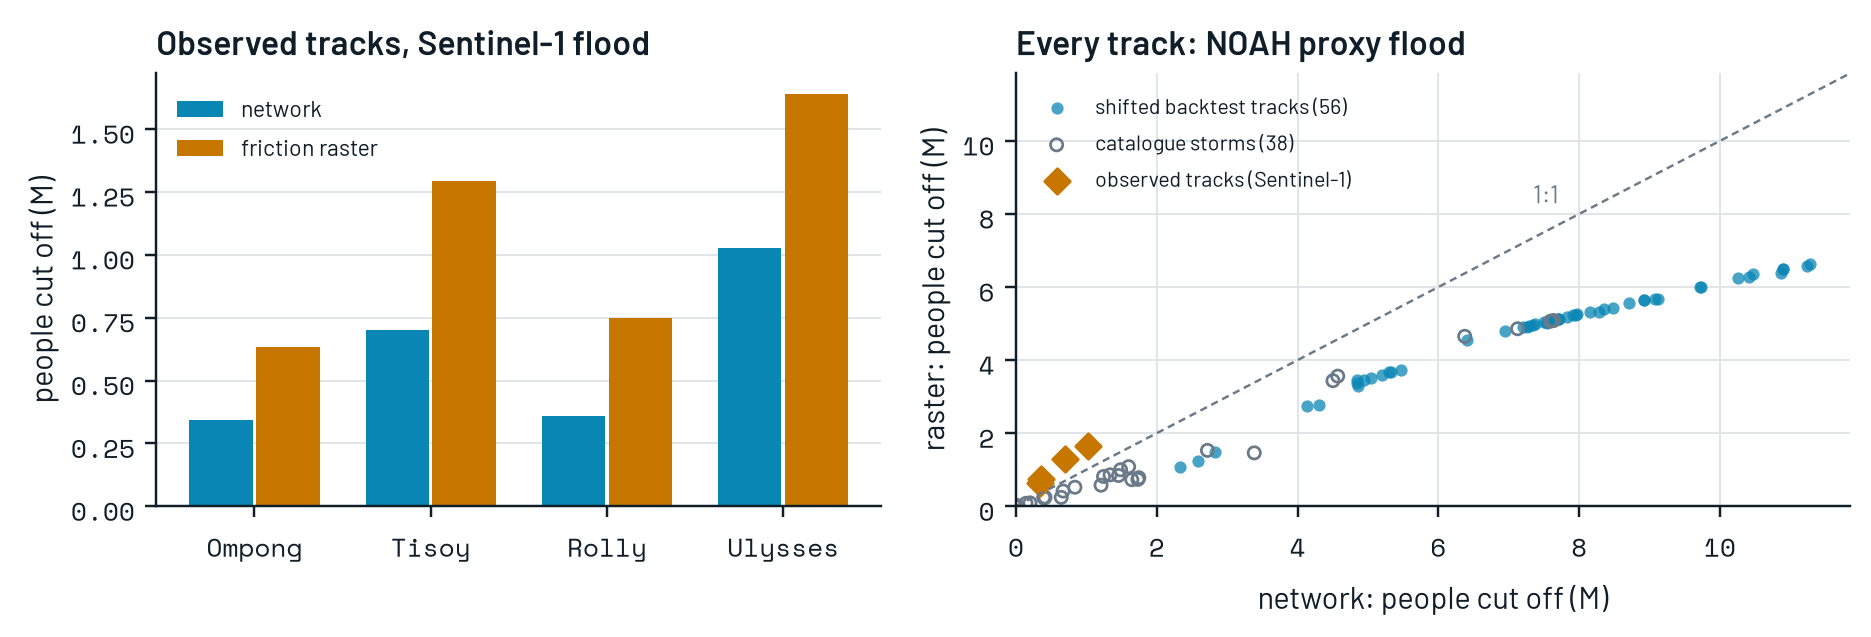
\includegraphics[width=\linewidth]{f15_methods}
\caption{People cut off by each method. Left: observed tracks with Sentinel-1 flood. Right: every track that uses the NOAH proxy (shifted backtest tracks and catalogue storms), with the 1:1 line.}
\label{fig:methods}
\end{figure}

\subsection{Vulnerable groups}

HRSL puts \uFiveShare{} of people under five and \oSixtyShare{} aged 60 or over; the 2020 census has \censusUFive{} and \censusSixty{}. \ifHRSLUnderOld HRSL therefore \textbf{under-counts older people}\ifHRSLOverYoung{} (and over-counts young children)\fi, so the 60+ cut-off numbers are low estimates.\fi{} Among those cut off, the under-5 share is \uFiveCutRange{} and the 60+ share \oSixtyCutRange{}.
